\chapter{The LHC and the CMS Detector}
\label{chap:cmsoverview}

Probing the \SM for signs of new physics would not be possible without the immensely complex electronics and machinery that makes the TeV energy scale accessible for the first time. This chapter will cover \CERN 's  Large Hadron Collider (\LHC) and the CMS detector, being the experiment the author is a member of. Section \ref{sec:cmsdetector} serves to introduce an overview of the different components of  the CMS detector, with more detail spent on those that are relevant in the search for Supersymmetric particles. Section \ref{sec:cmsobjects} will focus on event and object reconstruction again with more emphasis on jet level quantities which are most relevant to the author's analysis research. Finally Section \ref{sec:triggersystem} will cover work performed by the author, as service to the CMS Collaboration, in measuring the performance of the GCT component of the L1 trigger during the 2012-2013 run period.  


\section{The LHC}
\label{sec:thelhc} 

The \LHC is a storage ring, accelerator, and collider of circulating beams of protons or ions. Housed in the tunnel dug for the Large Electron-Positron collider (LEP), it is approximately 27 km in circumference, 100 m underground, and straddles the border between France and Switzerland outside of Geneva. It is currently the only collider in operation that is able to study physics at the TeV scale.  A double-ring circular synchrotron, it was
designed to collide both proton-proton (pp) and heavy ion (PbPb) with a centre of mass energy $\sqrt{s} = $ 14 \TeV at a final design luminosity of $10^{34}$cm$^{-2}$s$^{-1}$. \\

These counter-circulating beams of protons/Pb ions are merged in four sections around the ring to enable collisions of the beams, with each interaction point being home to one of the four major experiments; ALICE \cite{alicetdr} , ATLAS \cite{atlastdr}, CMS \cite{cmstdr} and LHCb \cite{lhcbtdr} which record the resultant collisions. The layout of the \LHC ring is shown in Figure \ref{fig:lhc-ring}. The remaining four sections contain acceleration,collimation and beam dump systems. In the eight arc sections, the beams are steered by magnetic fields of up to 8 \T provided by super conduction dipole magnets, which are maintained at temperatures of 2 \K using superfluid helium. Additional magnets for focusing and corrections are also present in straight sections within the arcs and near the interaction regions where the detectors are situated. \\


\begin{figure}[!h]

\centering
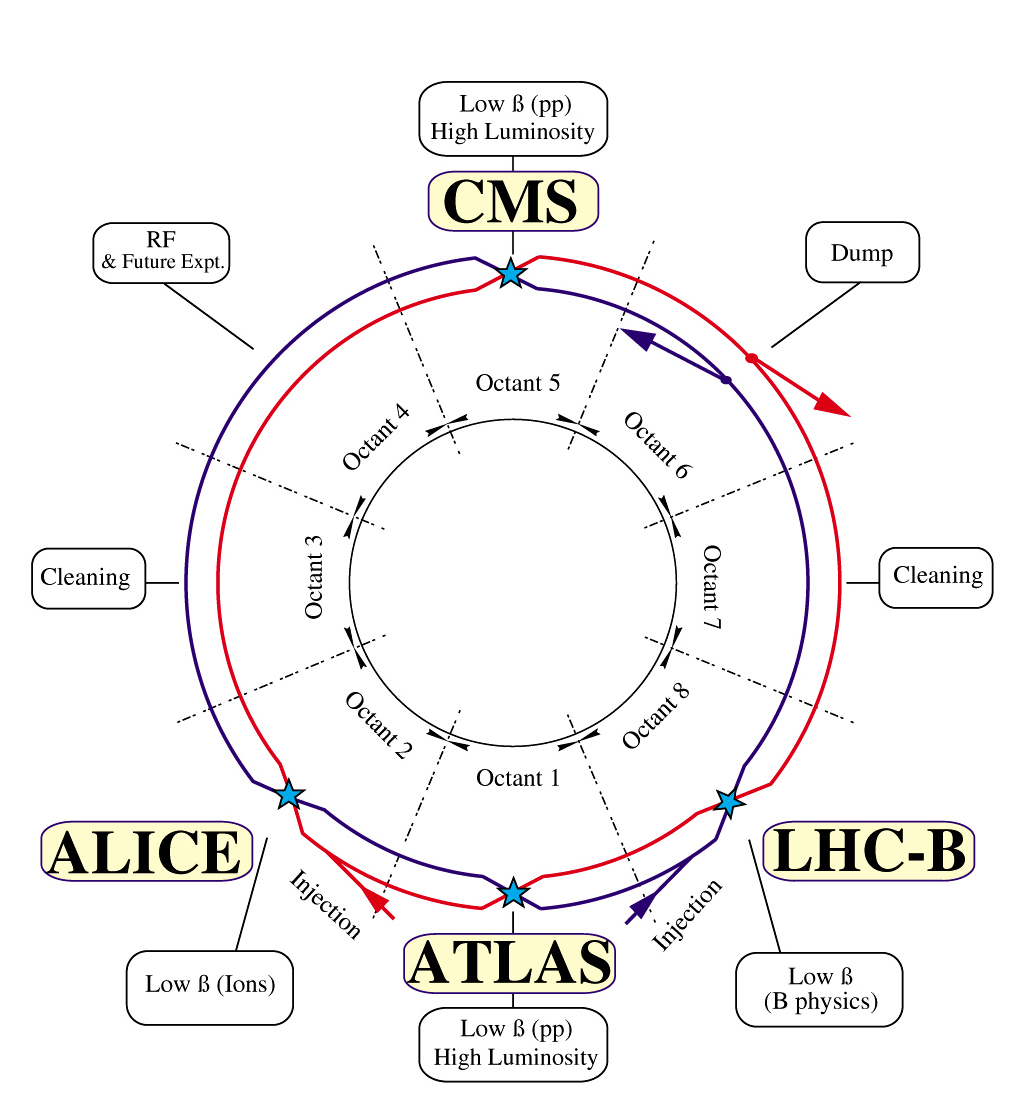
\includegraphics[width=0.65\textwidth]{plots/lhc-ring-photo.png}
\caption[A top down layout of the \LHC.]{A top down layout of the \LHC. \cite{Jean-Luc:841573}}  
\label{fig:lhc-ring}
\end{figure}


Proton beams are formed inside the Proton Synchrotron (PS) from bunches of protons 50 \ns apart with an energy of 26 \GeV. The protons are then accelerated in the Super Proton Synchrotron(SPS) to 450 \GeV  before being injected into the \LHC. These \LHC proton beams consists of many "bunches" i.e. approximately $1.1 \times 10^{11}$  protons localized into less than 1 \ns in the direction of motion. Before collision the beams are ramped to 4 \TeV (2012) per beam in a process involving increasing the current passing through the dipole magnets. Once the desired \com energy is reached then the beams are allowed to collide at the interaction points. The luminosity falls regularly as the run progresses as protons are lost in collisions, and eventually the beam is dumped before repeating the process again. \\

In the early phase of prolonged operation after the initial shutdown the machine operated in 2010-2011 at 3.5 \TeV per beam, \com $=$ 7 \TeV, delivering 6.13 \fb of data \cite{LHClumo}. During the 2012-2013 run period, data was collected at an increased \com $=$ 8 \TeV improving the sensitivity of searches for new physics. Over the whole run period 23.3 \fb of data was delivered of which 21.8 \fb was recorded by the \CMS detector \cite{LHClumo}. A total of 12 \fb of 8 \TeV certified data was collected by October 2012, and it is this data which forms the basis of the results discussed within this thesis.

\begin{figure}[!h]

\centering
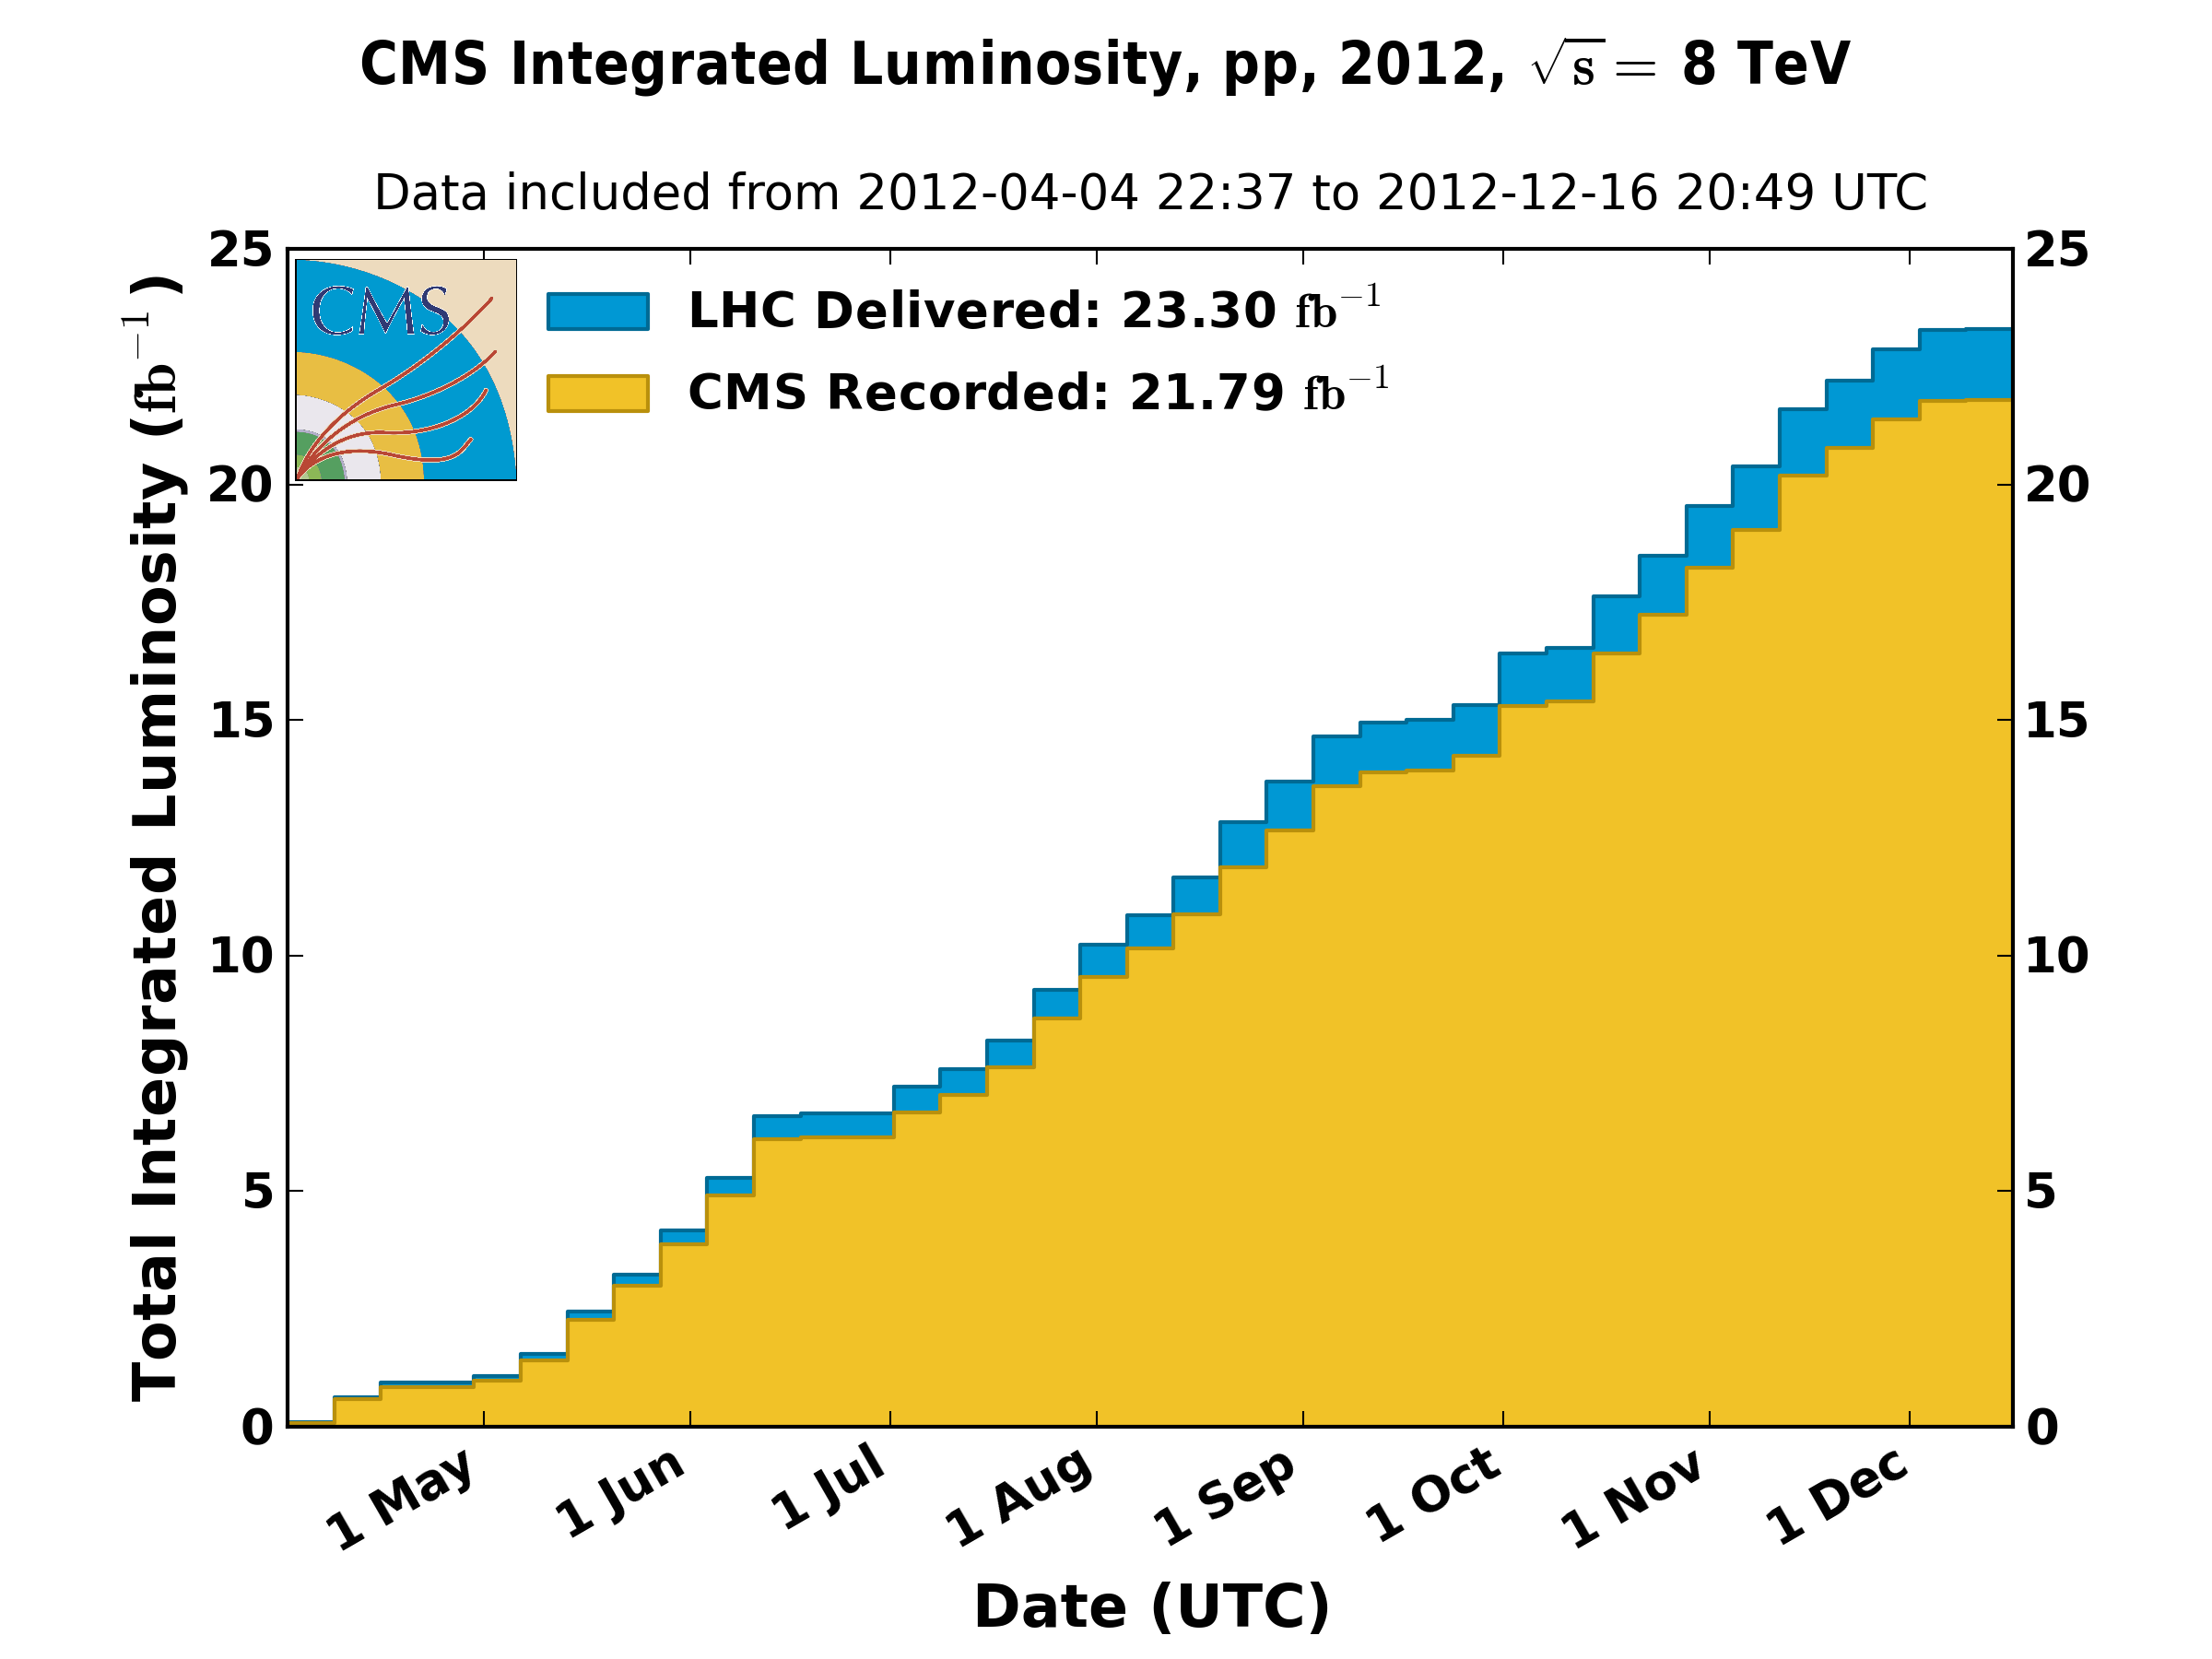
\includegraphics[width=0.65\textwidth]{plots/lhc-lumo-8tev.png}
\caption[The total integrated luminosity delivered to and collected by \CMS during the 2012 8 \TeV \pp runs]{The total integrated luminosity delivered to and collected by \CMS during the 2012 8 \TeV \pp runs.}  
\label{fig:lhc-ring}
\end{figure}


\section{The CMS detector}
\label{sec:cmsdetector}

The Compact Muon Solenoid (\CMS) detector is one of two general purpose detectors at the \LHC designed to search for new physics. The detector is designed to provide efficient identification and measurement of many physics objects including photons, electrons, muons, taus, and hadronic showers over wide ranges of transverse momentum and direction. Its nearly 4$\pi$ coverage in solid angle allows for accurate measurement of global transverse momentum imbalance. These design factors give \CMS the ability to search for direct production of \SUSY particles at the \TeV scale, making the search for Supersymmetric particles one of the highest priorities among the wide range of physics programmes at \CMS. \\

\CMS uses a right-handed Cartesian coordinate system with the origin at the interaction point and the z-axis pointing along the beam axis, the x-axis points radially inwards to the centre of the collider ring, with the y-axis points vertically upward. The azimuthal angle, $\phi$ ranging between [$-\pi$,$\pi$] is defined in the x-y plane starting from the x-axis. The polar angle $\theta$ is measured from the z axis. The common convention in particle physics is to express an out going particle in terms of $\phi$ and its pseudorapidity defined as

\begin{equation}
\eta = -\log\tan\left(\frac{\theta}{2}\right).
\end{equation}

The variable $\Delta R = \sqrt{\Delta\phi^{2} + \Delta\eta^{2} } $ is commonly used to define angular distance between objects within the detector and additionally energy and momentum is typically measured in the transverse plane perpendicular to the beam line. These values are calculated from the x and y components of the object and are denoted as $\et = E\sin\theta$ and $\pt = \sqrt{p^{2}_{x}+p^{2}_{y}}$. 

\subsection{Detector Subsytems}
\label{subsec:detectorsubsystems}

As the range of particles produced in \pp collisions interact in different ways with matter, \CMS is divided into subdetector systems, which perform complementary roles to identify the identity, mass and momentum of the different physics objects present in each event. These detector sub-systems contained inside \CMS are wrapped in layers around a central 13 m long 4 \T super conducting solenoid as shown in Fig \ref{fig:cms-detector}. With the endcaps closed , \CMS is a cylinder of length 22 m, diameter 15 m, and mass 12.5 kilotons. A more detailed complete description of the detector can be found elsewhere \cite{cmstdr}. \\

\begin{figure}[!h]

\centering
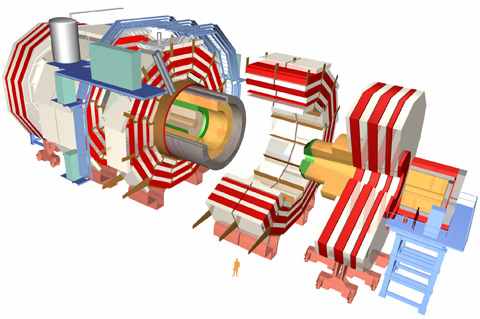
\includegraphics[width=0.65\textwidth]{plots/cms-detector.png}
\caption[A pictorial depiction of the \CMS detector.]{A pictorial depiction of the \CMS detector with the main detector subsystems labelled.   \cite{cms-public-detector}}  
\label{fig:cms-detector}
\end{figure}

\subsection{Tracker}
\label{subsec:tracker}

 The inner-most subdetector of the barrel is the multi-layer silicon tracker, formed of a pixel detector component encased by layers of silicon strip detectors. The pixel detector consists of three layers of silicon pixel sensors providing measurements of the momentum, position coordinates of the charged particles as they pass, and the location of primary and secondary vertices between 4cm and 10cm transverse to the beam. Outside the pixel detector, ten cylindrical layers of silicon strip detectors extend the tracking system out to a radius of 1.20m from the beam line. The tracking system provides efficient and precise determination of the charges, momenta, and impact parameters of charged particles with the geometry of the tracker extending to cover a rapidity range up to $\lvert\eta\rvert \textless$ 2.5.  \\
 
 The tracking system also plays a crucial part in the identification of jets originating from b-quarks through measurement of displaced secondary vertices, which is covered in more detail in Section \ref{subsec:cmsobjects-btagging}. The identification of b-jets is important in many searches for natural \SUSY models and forms an important part of the inclusive search strategy described within Section \ref{subsec:searchstrategy}.
 
\subsection{Electromagnetic Calorimeter}
\label{subsec:ecal}

 Immediately outside of the tracker, but still within the magnet core, sits the Electromagnetic Calorimeter (\ECAL). Covering a pseudorapididity up to $\lvert\eta\rvert < 3$ and compromising of over 75,000 PbWO$_{4}$ (lead tungstate) crystals that scintillate as particles deposit energy, the \ECAL provides high resolution measurements of the electromagnetic showers from photons, electrons in the detector. \\ 
 
 Lead tungstate is used because of its short radiation length ($X_{0} \sim 0.9$cm) and small Molier\'{e} radius ($\sim 2.1$cm) leading to high granularity and resolution. It's fast scintillation time ($\sim 25$ns) reduces the effects of pileup due to energy from previous collisions still being read out, and its radiation hardness gives it longevity. The crystals are arranged in modules which surround the beam line in a non-projective geometry,  angled at 3$^{\circ}$ with respect to the interaction point to minimise the risk of particles escaping down the cracks between the crystals.\\
 
 The  \ECAL is primarily composed of two sections, the Electromagnetic Calorimeter Barrel (\EB) which extends in pseudo-rapidity to $\lvert\eta\rvert < 1.479$ with a crystal front cross section of 22 $\times$ 22 mm$^{2}$ and a length of 230 mm corresponding to 25.8 radiation lengths, and the Electronmagnetic Calorimeter Endcaps (\EE) covering a rapidity range of $1.479 < \lvert\eta\rvert < 3.0 $, which consists of two identical detectors
on either side of the EB.  A lead-silicon sampling `pre-shower' detector (\ES) is placed before the endcaps to aid in the identification of neutral pions. Their arrangement are shown in Figure \ref{fig:cms-ecal}. \\

 
 \begin{figure}[!h]

\centering
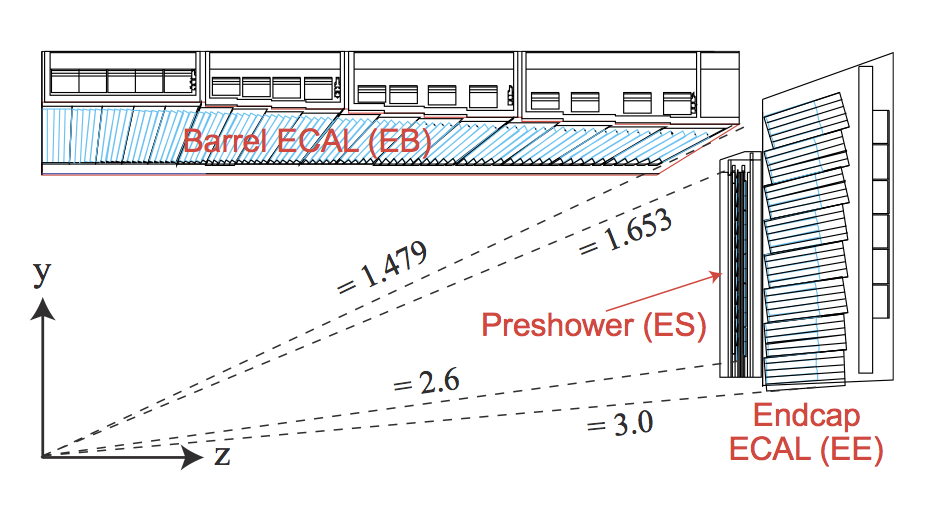
\includegraphics[width=0.85\textwidth]{plots/cms-ecal.png}
\caption[Illustration of the \CMS \ECAL showing the arrangement of the lead tungstate crystals in the \EB and \EE. The \ES is also shown and is located infront of the \EE.]{Illustration of the \CMS \ECAL showing the arrangement of the lead tungstate crystals in the \EB and \EE. The \ES is also shown and is located infront of the \EE \cite{CMS_ECAL_TDR}.}  
\label{fig:cms-ecal}
\end{figure}


Scintillation photons from the lead tungstate crystals are instrumented with avalanche photo-diodes (\APD) and vacuum photo-triodes (\VPT) located in the \EB and \EE respectively, converting the scintillating light into an electric signal which is consequently used to determine the amount of energy deposited within the crystal . These instruments are chosen for their resistance under operation to the strong magnetic field of \CMS. The scintillation of the \ECAL crystals as well as the response of the \APD s varies as a function of temperature and so cooling systems continually maintain an overall constant \ECAL temperature $\pm 0.05 ^{\circ}C$.
 

\subsection{Hadronic Calorimeter}
\label{subsec:hcal} 

Beyond the \ECAL lies the Hadronic Calorimeter (\HCAL), which is responsible for the accurate measurement of hadronic showers, crucial for analyses involving jets or missing energy signatures. The \HCAL is a sampling calorimeter which consists of alternating layers of brass absorber and plastic scintillator, except in the hadron forward ($3.0 < \lvert\eta\rvert < 5.0 $) region in which steel absorbers and quartz fibre scintillators are used because of their increased radiation tolerance. Hadron showers are initiated in the absorber layers inducing scintillation in the plastic scintillator tiles.  These scintillation photons are converted by wavelength shifting fibres for read-out by hybrid photodiodes. \\

The \HCAL's size is constrained to a compact size by the presence of the solenoid, requiring the placement of an additional outer calorimeter on the outside of the solenoid to increase the sampling depth of the \HCAL. A schematic of the \HCAL can be seen in Figure \ref{fig:cms-hcal}.\\
 
 \begin{figure}[!h]

\centering
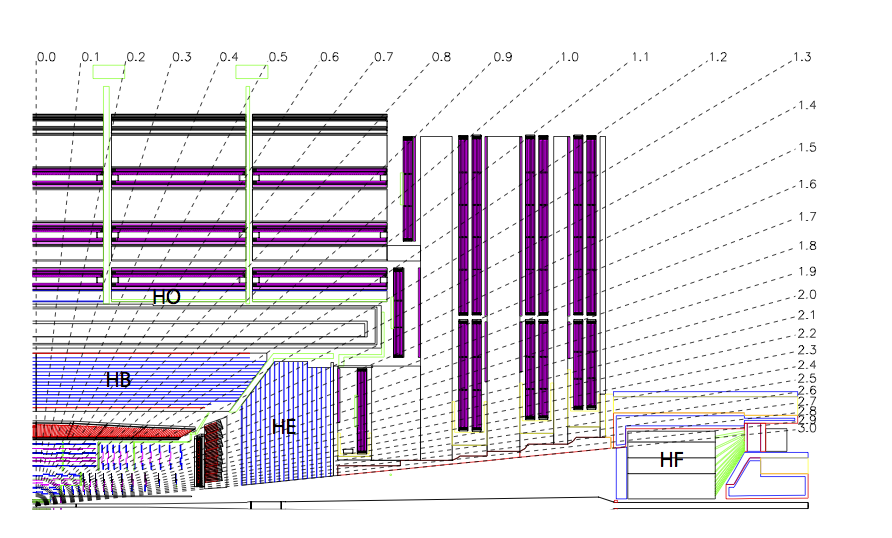
\includegraphics[width=0.85\textwidth]{plots/cms-hcal.png}
\caption[Schematic of the hadron calorimeters in the r-z plane, showing the locations of the HCAL components and the HF]{ Schematic of the hadron calorimeters in the r-z plane, showing the locations of the HCAL components and the HF. \cite{cmstdr}.}  
\label{fig:cms-hcal}
\end{figure}
 
The HCAL covers the range $\lvert\eta\rvert < 5$ and consists of four subdetectors: the Hadron Barrel (\HB)  $\lvert\eta\rvert < 1.3$, the Hadron Outer (\HO), the Hadron Endcap (\HE) $1.3 < \lvert\eta\rvert < 3.0 $ and the Hadron Forward (\HF).  The \HB is contained between the outer edge of the \ECAL and the inner edge of the solenoid, formed of 36 azimuthal wedges it is split between two half-barrel segments. The relatively short number of interaction lengths ($\lambda_{l}$, the distance a hadron will travel through the absorber material before it has lost $\frac{1}{e}$ of its energy) within the \HB, the lowest being $\lambda_{l}$ = 5.82 for $\lvert\eta\rvert = 0$, facilitates the need for the `tail catching' \HO to increase the sampling depth in the central barrel rapidity region $\lvert\eta\rvert < 1.3$ to 11 interaction lengths . Significant fractions of the hadrons energy will be deposited in the \ECAL as it passed through the detector. Therefore measurements of hadron energies in the central regions $\lvert\eta\rvert < 3.0$ use both the \ECAL and \HCAL to reconstruct the true energy from showering hadrons. 

\subsection{Muon Systems}
\label{subsec:muonsystems} 
 
Muons being too massive to radiate away energy via Bremsstrahlung, interact little in the calorimeters and mostly pass through the detector until they reach the system of muon detectors which forms the outer most part of the \CMS detector.  

Outside of the superconducting solenoid are four muon detection layers interleaved with the iron return yokes which measure the muons energy via ionisation of gas within detector elements. Three types of gaseous chamber are used. The drift tube (\DT), cathode strip chamber (\CSC), and resistive plate chamber (\RPC) systems provide efficient detection of muons with pseudo-rapidity $\lvert\eta\rvert < 2.4 $. The best reconstruction performance is obtained when the muon chamber is combined with the inner tracking information to determine muon trajectories and their momenta \cite{CMS_MUON_TDR}.  \\ 

\section{Event Reconstruction and Object Definition}
\label{sec:cmsobjects}

The goal of event reconstruction is to take the raw information recorded by the detector and to compute from it higher-level quantities which can be used at an analysis level. These typically correspond to an individual particle's energy and momenta, or groups of particles which shower in a narrow cone and the overall global energy and momentum balance of the event. The reconstruction of these objects are described in great detail in \cite{CMS_TDR_PHYS_vol1}, however covered below are brief descriptions of those which are most relevant to the analysis detailed in Section \ref{chap:SUSYsearches}.

\subsection{Jets}
\label{subsec:cmsobjects-jets}

Quarks and gluons are produced copiously at the LHC in the hard scattering of partons. As these quarks and gluons fragment, they hadronise and decay into a group of strongly interactive particles and their decay products. These streams of particles travel in the same direction, as they have been "boosted" by the momentum of the primary hadron. These collections of decay products are reconstructed and identified together as a ``jet''.

At \CMS jets are reconstructed from energy deposits in the detector using the anti-kt algorithm \cite{antiktalgo} with size parameter $\Delta R = 0.5$. The anti-kt jet algorithm clusters jets by defining a distance between hard (high $\pt$) and soft (low $\pt$) particles such that soft particles are preferentially clustered with hard particles before being clustered between themselves. This produces jets which are robust to soft particle radiation from the pileup conditions experienced at the \LHC. \\

There are two main type of jet reconstruction used at \CMS, Calorimeter and PF jets \cite{CMS-PAS-JME-10-003}. Calorimeter jets are reconstructed using both the electromagnetic (\ECAL) and hadronic (\HCAL) calorimeter cells, combined into calorimeter towers . These calorimeter towers consist of geometrically matched \HCAL cells and \ECAL crystals. Electronics noise is suppressed by applying a threshold to the calorimeter cells, with pile-up effects reduced by a requirement placed on the tower energy  \cite{Janssen:1322145}. Calorimter jets are the jets used within the analyses described in this thesis.  

PF jets are formed from combining information from all of the CMS subdetectors systems to  determine which final state particles are present in the event. Generally, any particle is expected to produce some combination
of a track in the silicon tracker, a deposit in the calorimeters, or a track in the muon system. The PF jet momentum and spatial resolutions are greatly improved with respect to calorimeter jets, as the use of the tracking detectors and of the high granularity of ECAL allows resolution and measurement of charged hadrons and photons inside a jet,  which together constitute $\sim$ 85$\%$ of the jet energy \cite{1748-0221-6-11-P11002}.

The jets reconstructed by the clustering algorithm in \CMS typically have an energy that differs to the `true' energy measured by a perfect detector. This stems from the non-linear and nonuniform response of the calorimeters as well as other residual effects including pileup and underlying events, and therefore additional corrections are applied to recover a uniform relative response as a function of pseudo-rapidity. These are applied as separate sub corrections \cite{1742-6596-404-1-012014}. 

\begin{itemize}

\item A PU correction is first applied to the jet. It subtracts the average extra energy deposited in the jet that comes from other vertices present in the event and is therefore not part of the hard jet itself.
\item $\pt$ and $\eta$ dependant corrections derived from Monte Carlo simulations are used to account for the non-uniform response of the detector.\item $\pt$ and $\eta$ residual corrections are applied to data only to correct for difference between data and Monte Carlo. The residual is derived from QCD dijet samples and the $\pt$ residual from $\gamma + $ jet and $Z + $ jets samples in data.

\end{itemize}

\subsection{B-tagging}
\label{subsec:cmsobjects-btagging}

The decays of b quarks are suppressed by small \CKM matrix elements. As a result, the lifetimes of b-flavoured hadrons, produced in the fragmentation of b quarks, are relatively long; $\mathcal{O}$ 1ps. The identification of jets origination from b quarks is very important for searches for new physics and for measurements of standard model processes.  \\

Many different algorithms developed by CMS select b-quark jets based on variables such as the impact parameters of the charged-particle tracks, the properties of reconstructed decay vertices, and the presence or absence of a lepton, or combinations thereof. One of the most efficient of which is the Combined Secondary Vertex (\CSV) which operates based on secondary vertex and track-based lifetime information, benchmarked in `Loose', `Medium' and `Tight' working points, of which the medium point is the tagger used within the \alphat search detailed in Section \ref{sec:alphatintroduction}.

Using the \CSV tagger, a likelihood-based discriminator distinguishes between jets from b-quarks, and those from charm or light quarks and gluons, which is shown in Figure \ref{fig:btagdescrims}. The minimum thresholds on the discriminator for each working point correspond to the misidenti�cation probability for light-parton jets of 10$\%$, 1$\%$, and 0.1$\%$, respectively, in jets with an average $\pt$ of about 80 \GeV. 

\begin{figure}[ht]
\centering
\begin{minipage}[b]{0.55 \linewidth}
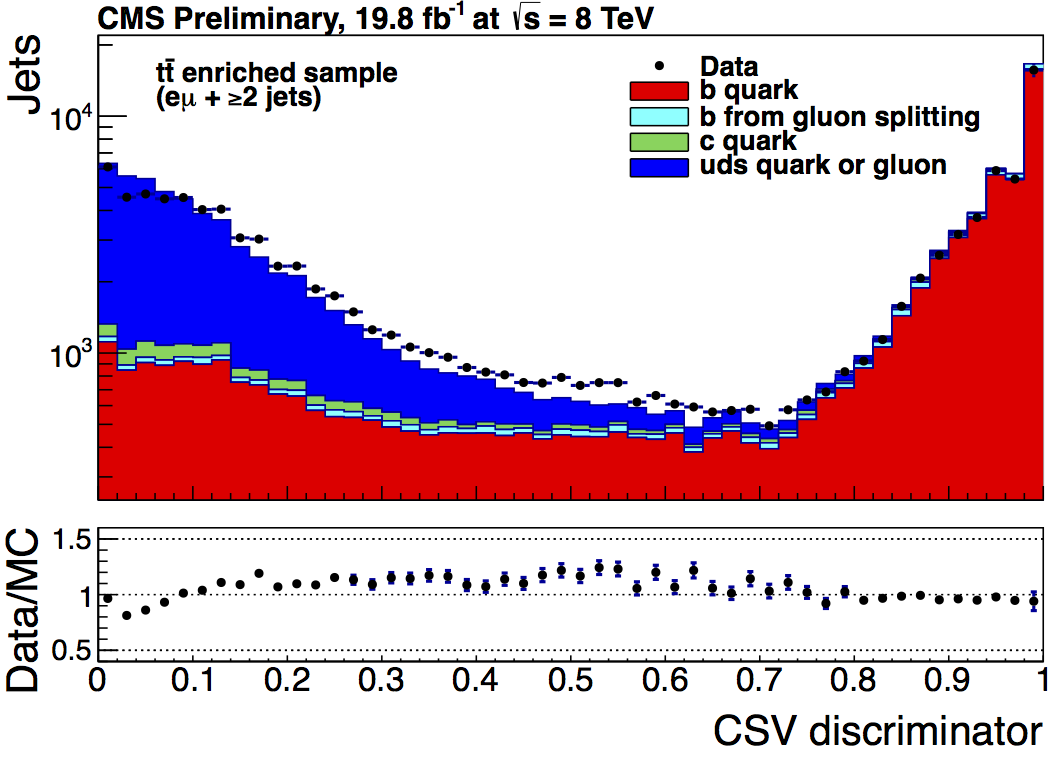
\includegraphics[width = 1.0\linewidth]{plots/btag-ttbardiscrim.png}
\end{minipage}
\quad
\begin{minipage}[b]{0.55\linewidth}
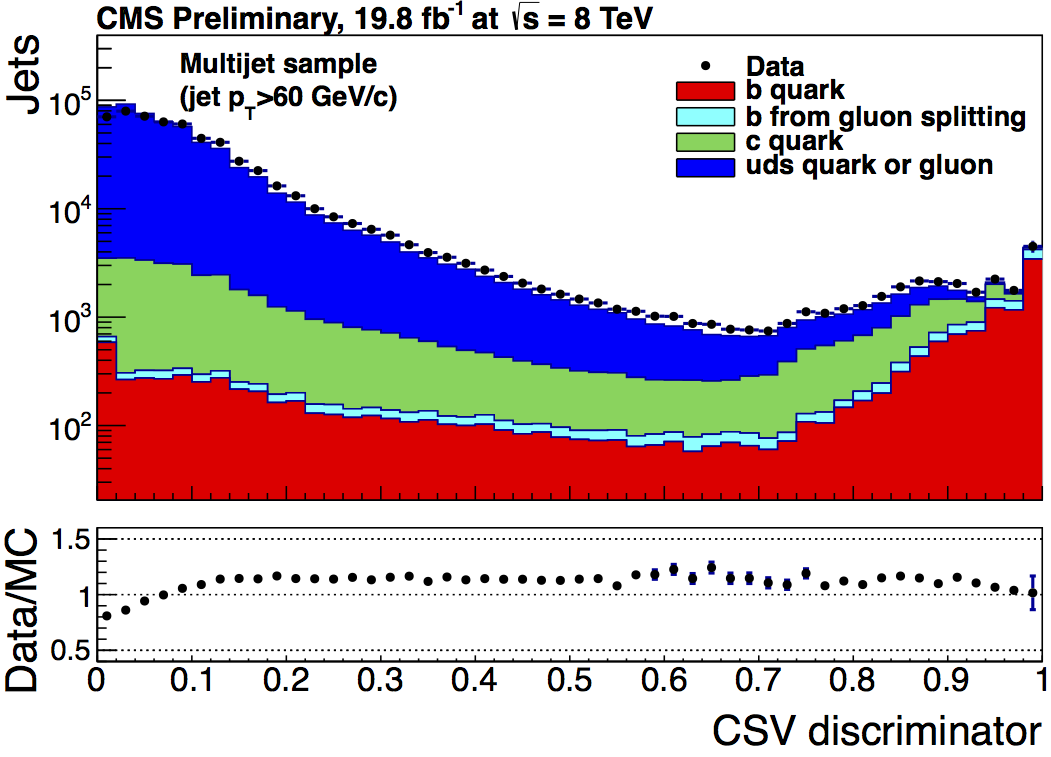
\includegraphics[width = 1.0\linewidth]{plots/btag-multijetdiscrim.png}
\end{minipage}
\caption[CSV algorithm discriminator values in enriched ttbar and inclusive multi jet samples]{CSV algorithm discriminator values in enriched ttbar (top) and inclusive multi jet samples (bottom) for b,c and light flavoured jets \cite{btag8tev}. Working points are determined from the misidentification probability for light-parton jets to be tagged as a b-jet and are given as 0.244, 0.679 and 0.898 for L,M and T working points respectively. }
\label{fig:btagdescrims}
\end{figure}

The b-tagging performance is evaluated to measure the b-jet tagging efficiency \effb, and the misidentification probability of charm \effc and light-parton jets \effs . The tagging efficiencies for each of these three jet flavours are compared between data and MC simulation, from which a series of $\pt$ and $\lvert\eta\rvert$ binned jet corrections are determined,

\begin{equation}
SF_{b,c,s} = \frac{\epsilon^{data}_{b,c,s}}{\epsilon^{MC}_{b,c,s}} .
\end{equation}

These are collectively named `Btag Scale Factors' and allow MC simulation to accurately reflect the running conditions and performance of the tagging algorithm in data. Understanding of the b-tagging efficiency is essential in order to minimise systematic uncertainties in physics analyses that employ b-tagging. \\
 
The b-tagging efficiency is measured in data using several methods applied to multi jet events, primarily based on a sample of jets enriched in heavy flavour content. One method requires the collection of events with a soft muon within a cone $\Delta R < 0.4$ around the jet axis. Because the semileptonic branching fraction of b hadrons is significantly larger than that for other hadrons, these jets are more likely to arise from b quarks than from another flavour, with the resultant momentum component of the muon transverse to the jet axis larger for muons from b-hadron decays than from light or charm jets.  Additionally the performance of the tagger can also be benchmarked in \ttbar events where in the \SM, the top quark is expected to decay to a W boson and a b quark about 99.8$\%$ of the time \cite{pdg2012}. Further selection criteria is applied to these events to further enrich the b quark content of these events. The methods to identify b-jets in data are discussed in great detail at \cite{btag7tev}. The jet flavours are determined in simulation using truth level information and are compared to data to determine the correction scale factors ($SF_{b}$), which are displayed for the CSVM tagger in Figure \ref{fig:btagscalefactors}. 

\begin{figure}[ht]
\centering
\begin{minipage}[b]{0.31 \linewidth}
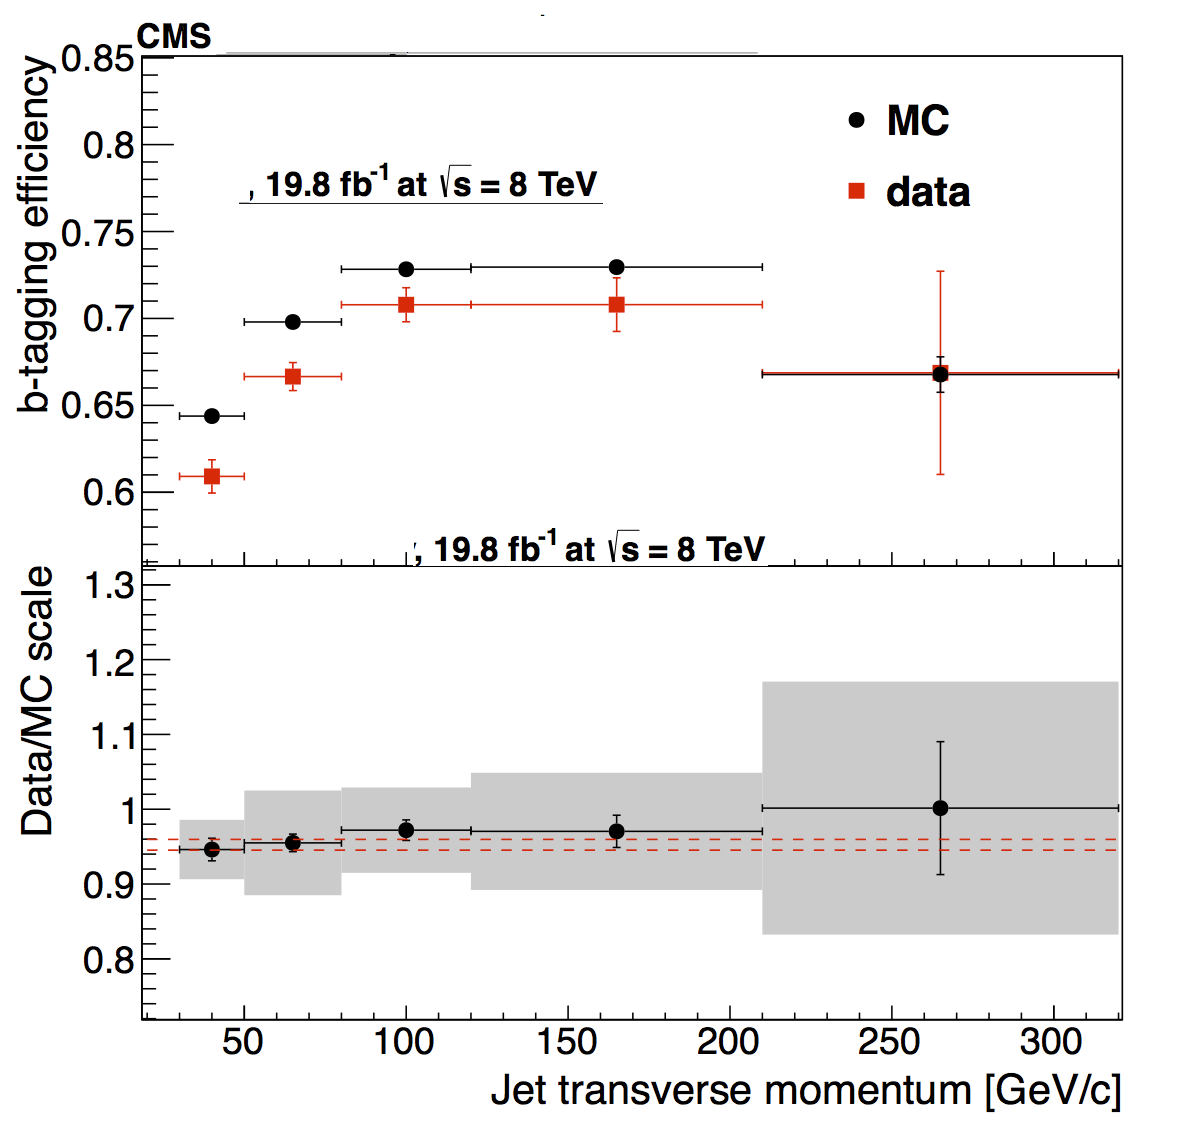
\includegraphics[width = 1.0\linewidth]{plots/btag-csvm_pt_sf.png}
\end{minipage}
\quad
\begin{minipage}[b]{0.31\linewidth}
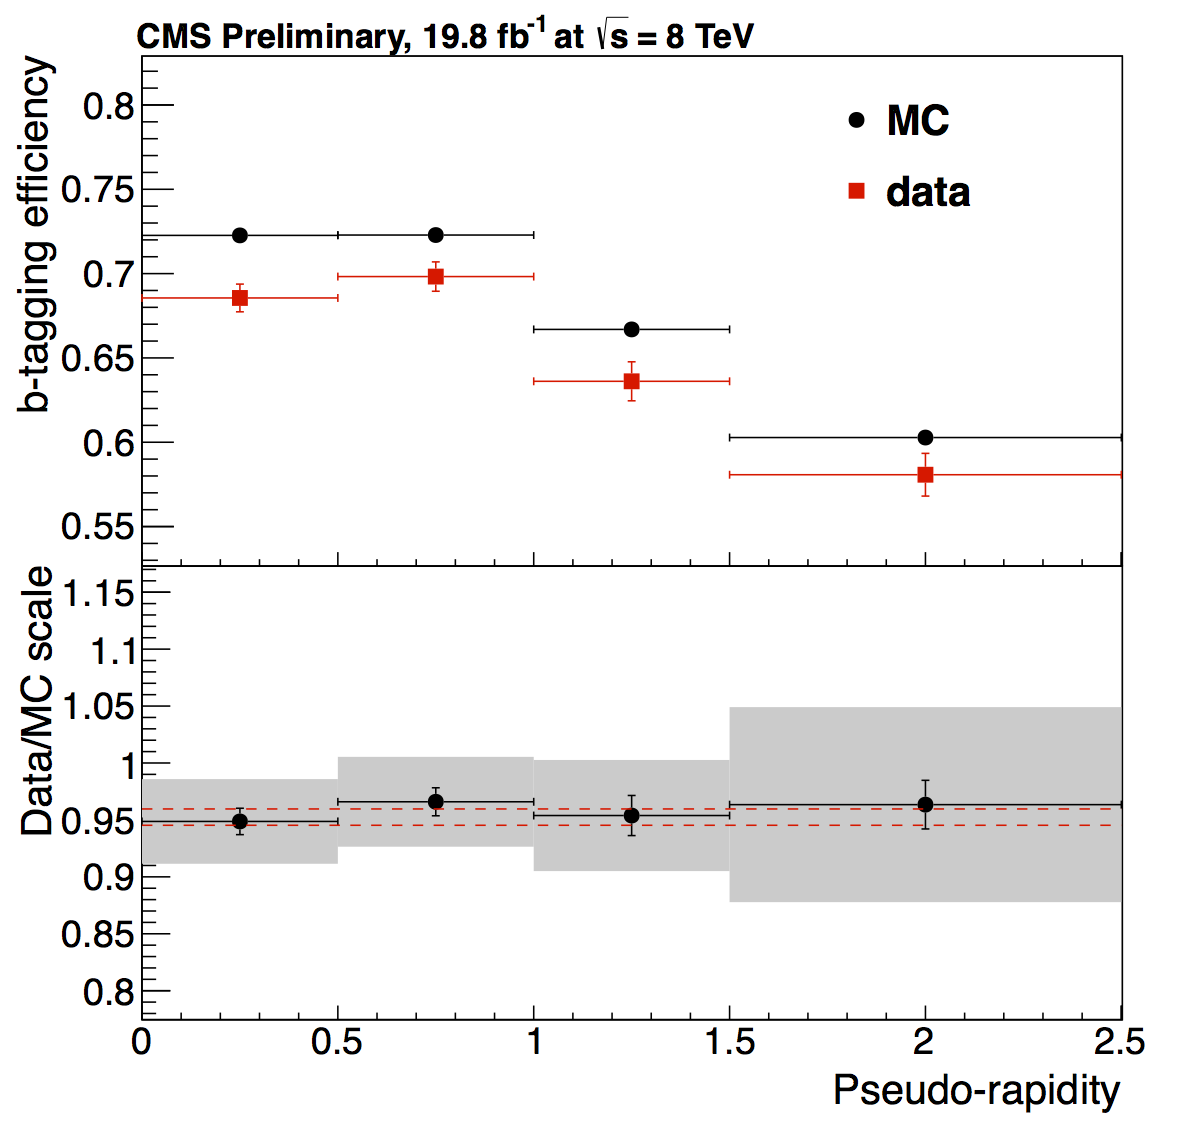
\includegraphics[width = 1.0\linewidth]{plots/btag-csvm_eta_sf.png}
\end{minipage}
\quad
\begin{minipage}[b]{0.31\linewidth}
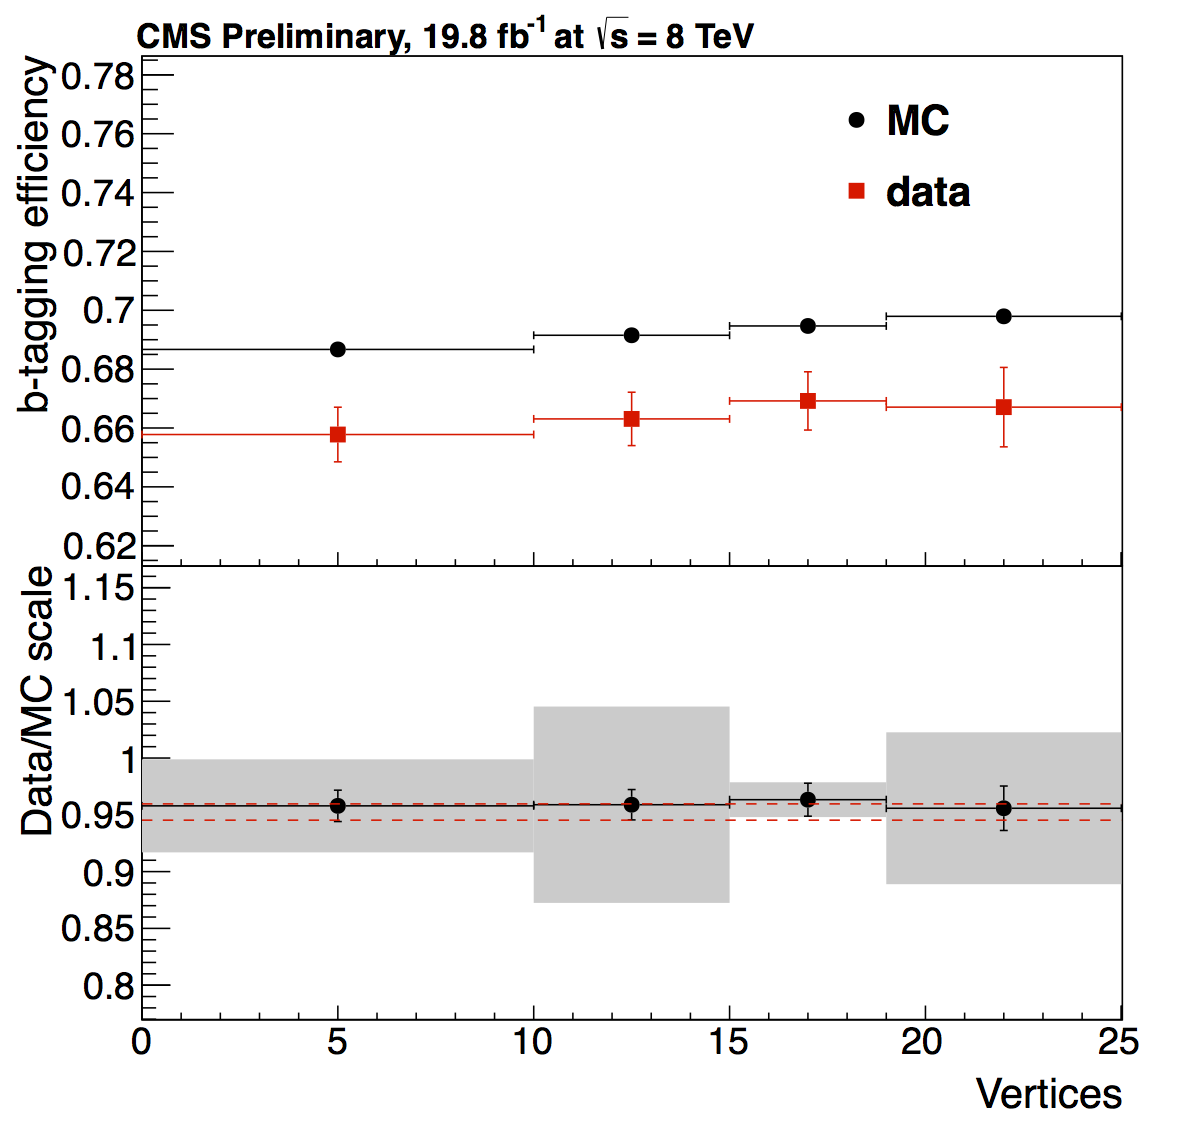
\includegraphics[width = 1.0\linewidth]{plots/btag-csvm_vert_sf.png}
\end{minipage}
\caption[Measured in \ttbar $\rightarrow$ di-lepton events using the CSVM tagger: (upper panels) b-tagging efficiencies and (lower panels) data/MC scale factor $SF_{b}$ as a function of (left) jet $\pt$, (middle) jet $\lvert\eta\rvert$ and (right) number of primary vertices. In the lower panels, the grey filled areas represent the total statistical and systematic uncertainties, whereas the dotted lines are the average $SF_{b}$ values within statistical uncertainties.]{Measured in \ttbar $\rightarrow$ di-lepton events using the CSVM tagger: (upper panels) b-tagging efficiencies and (lower panels) data/MC scale factor $SF_{b}$ as a function of (left) jet $\pt$, (middle) jet $\lvert\eta\rvert$ and (right) number of primary vertices. In the lower panels, the grey filled areas represent the total statistical and systematic uncertainties, whereas the dotted lines are the average $SF_{b}$ values within statistical uncertainties.}
\label{fig:btagscalefactors}
\end{figure}

The measurement of the misidenti�cation probability for light-parton jets relies on the inversion of tagging algorithms, selecting non-b jets using the same variables and techniques used in benchmarking the b-tagging efficiency. The scale factors ($SF_{s}$) to be applied to MC are shown in Figure \ref{fig:mistagscalefactors} for the CSVM tagger.

\begin{figure}[ht]
\centering
\includegraphics[width=0.80\textwidth]{plots/btag-csvmsf.png}
\caption[For the CVSM tagging criterion: (top) misidenti�cation probability in data (filledcircles) and simulation (open circles); (bottom) scale factor for the misidenti�cation probability. The last $\pt$ bin in each plot includes all jets with $\pt > 1000$ \GeV. The solid curve is the result of a polynomial fit to the data points. The dashed curves represent the overall statistical and systematic uncertainties on the measurements.]{For the CVSM tagging criterion: (top) misidenti�cation probability in data (filled circles) and simulation (open circles); (bottom) scale factor for the misidenti�cation probability. The last $\pt$ bin in each plot includes all jets with $\pt > 1000$ \GeV. The solid curve is the result of a polynomial fit to the data points. The dashed curves represent the overall statistical and systematic uncertainties on the measurements.}  

\label{fig:mistagscalefactors}
\end{figure}


\section{Triggering System}

\label{sec:triggersystem}

With bunch crossings separated by just 25 ns, the rate at which data from collisions would have to be written out and processed would be unfeasible. A two-tiered triggering system is applied at \CMS in order to cope with the high collision rate of protons. The \CMS trigger is designed to use limited information from each event to determine whether to record the event, reducing the rate of data taking to manageable levels whilst ensuring a high efficiency of interesting physics object events are selected.

The Level-1 (\L1) trigger is a pipelined, dead-timeless system based on custom-built electronics \cite{Dasu:2000ge}. The \L1 system is covered in more detail within the following section along with a description of the service work undertaken by the author to benchmark the performance of the \L1 calorimeter trigger during the 2012 8 \TeV run period.

The Higher Level Trigger (\HLT) is a large farm of commercial computers \cite{Sphicas:2002gg}. The \HLT processes events with software reconstruction algorithms that are closer to the reconstruction used offline. The \HLT provides a rejection factor of approximately 500, reducing the event rate to disk to just a few hundred per second. The recorded events are transferred from CMS to the CERN computing center, where event reconstruction is performed, and then distributed to CMS computing sites around the globe for storage and analysis.

\subsection{\L1 Trigger}
\label{subsec:l1trigger}

In the Level-1 calorimeter trigger, coarse measurements of the energy deposited in the electromagnetic and hadronic calorimeters are combined and by using sophisticated algorithms the following physics objects are formed:

\begin{itemize}
	\item isolated and non-isolated electromagnetic objects (electrons and photons);
	\item hadronic jets in the central and forward sections of the hadronic calorimeters;
	\item hadronically decaying tau leptons;
	\item total transverse energy ($\et$) and missing transverse energy ($\met$); 
	\item total transverse jet energy ($\theht$) and missing transverse jet energy ($\mht$). 
\end{itemize}

In addition quantities suitable for triggering minimum bias events, forward physics and beam background events are calculated. With the exception of the electromagnetic objects all the \L1 calorimeter trigger algorithms run in the Global Calorimeter Trigger (\GCT) hardware.


\subsection{ \L1 Trigger Jet Algorithm}
\label{subsec:l1jettrigger}

The \L1 jet trigger uses the transverse energy sums computed in the calorimeter (both hadronic and electromagnetic) trigger regions. Each region consists of $4 \times 4 $  trigger tower windows, spanning a region of $\Delta \eta \times \Delta \phi = 0.087 \times 0.087$ in pseudorapidity-azimuth. The jet trigger uses a $3 \times 3$ calorimeter region (112 trigger towers) sliding window technique which spans the full $(\eta, \phi)$ coverage of the CMS calorimeter (Fig.~\ref{fig:l1jetalgo}). In forming a \L1 jet is it required that the central region to be higher than the eight neighbouring regions $ E_{T central} > E_{T surround}$, and also be higher than a minimum threshold of 1 \GeV (This was increased to 5 \GeV during the 2012 run period. The effects of which are shown in Section \ref{subsec:l1jetseedpu}), the latter to suppress noise . 

The L1 jets are characterised by the $\et$, summed over the $3 \times 3$ calorimeter regions, which corresponds to $12 \times 12$ trigger towers in barrel and endcap or $3 \times 3$ larger \HF towers in the \HF. The $\phi$ size of the jet window is the same everywhere, whilst the $\eta$ binning gets somewhat larger at high $\eta$ due to calorimeter and trigger tower segmentation. The jets are labelled by $(\eta, \phi)$ indexes of the central calorimeter region.                                                                                                                                                  

Jets with $|\eta|>3.0$ are classified as forward jets, whereas those with $|\eta|<3.0$ are classified as central. The four highest energy central and forward jets in the calorimeter are selected. After jets are found, Look Up Tables (\LUT's) are used to apply a programmable $\eta-$dependent jet energy scale correction. 

\begin{figure}[ht!]
\centering
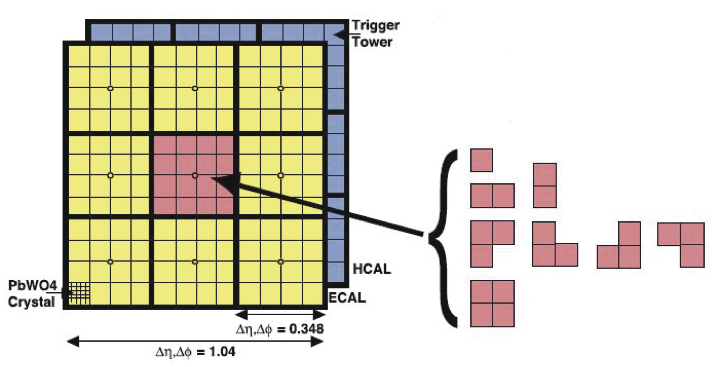
\includegraphics{plots/L1JetAlgorithm.png}
\caption[Illustration of the Level-1 jet finding algorithm.]{Illustration of the Level-1 jet finding algorithm.}  
\label{fig:l1jetalgo}
\end{figure}  


\subsection{Measuring \L1 Jet Trigger Efficiencies}
\label{subsec:l1jettrigeff}

Measurement of the \L1 trigger efficiency is essential for �.  

The L1 jet efficiency is defined as the fraction of leading offline jets which were matched with a L1 tau or central jet above a certain trigger threshold, divided by all the offline jets in the event. This quantity is then plotted as a function of the offline jet $\et$, $\eta$ and $\phi$. The efficiency is determined by matching the \L1 and reconstructed offline jets spatially in $\eta - \phi$ space.  This is done by calculating the minimum separation in $\Delta R$ between the highest offline reconstructed jet in $\et$ ($\et>10$~GeV,$\lvert\eta\rvert<3$) and any L1 jet. A jet will be matched if this value is found to be $< 0.5$. Should more than one jet satisfy this, the jet closest in $\Delta R$ is taken as the matched jet.

\subsection{Effects of the \L1 Jet Seed and Robustness to Pileup}
\label{subsec:l1jetseedpu}

Between run B and run C of the 2012 data taking period, a jet seed threshold was introduced into the \L1 trigger jet algorithm. The jet seed was introduced to counteract the effects of high pile up running conditions which create a large number of soft non-collimated jets, that are then added to the jets from the primary interaction or other soft jets from other secondary interactions. This in turn causes a large in trigger rate due to the increase in the likelihood that the event causes the \L1 trigger to fire.




